\documentclass[12pt,a4paper]{report}
\setlength{\headheight}{15pt}
\usepackage[utf8]{inputenc}
\usepackage{comment}
\usepackage[T1]{fontenc}
\usepackage[italian]{babel}
\usepackage{graphicx}
\usepackage{hyperref}
\usepackage{amsmath}
\usepackage{booktabs}
\usepackage{lipsum}
\setlength{\headheight}{27pt}
\usepackage[backend=biber,style=authoryear]{biblatex}
\setlength{\bibitemsep}{12pt}
\usepackage{csquotes}

% Pacchetti necessari
\usepackage{geometry}
\usepackage{fancyhdr}
\usepackage{tikz}
\usepackage{float}
\usetikzlibrary{shapes, arrows.meta, positioning}
\addbibresource{bibliography.bib}

% Margini
\geometry{a4paper, top=3cm, bottom=3cm, left=2.5cm, right=2.5cm}

% Header/Footer
\pagestyle{fancy}
\fancyhf{}
\rhead{\thepage}
\lhead{\leftmark}

% Impostazioni corpo testo e citazioni
\renewcommand{\normalsize}{\fontsize{12pt}{14pt}\selectfont}
\renewcommand{\footnotesize}{\fontsize{10pt}{12pt}\selectfont}
\renewenvironment{quote}{\list{}{\rightmargin=1cm \leftmargin=1cm}\item\relax\fontsize{11pt}{13pt}\selectfont}{\endlist}

\setcounter{secnumdepth}{3}

\begin{document}

% Frontespizio
\begin{titlepage}
    \begin{center}
        \textsc{\LARGE Universit\`a degli Studi eCampus} \\
        \vspace{0.5cm}
        \textsc{\Large Tesi di Laurea} \\
        \vspace{1.5cm}

        {\Huge \textbf{Domotica Residenziale}} \\
        \vspace{0.5cm}
        {\Large \textbf{Evoluzione dei Protocolli di Comunicazione IoT e}} \\
        \vspace{0.2cm}
        {\Large \textbf{Gestione di Dispositivi Multimarca}} \\

        \vfill
        \begin{flushleft}
            \textbf{Relatore:} Prof. Christian Callegari \\
            \textbf{Candidato:} Michele Rota Biasetti \\
            Matricola n\textsuperscript{o} 1518870
        \end{flushleft}

        \vfill
        Anno accademico 2024/2025
    \end{center}
\end{titlepage}

% Indice
\tableofcontents
\newpage

% Capitolo 1: Introduzione
\chapter{Introduzione}
Negli ultimi anni, le tecnologie legate all'Internet of Things, o IoT, hanno fatto davvero tanta strada. Oggi si trovano praticamente ovunque e hanno cambiato il modo in cui viviamo la casa. Non si parla più solo di pareti e mobili: l'abitazione diventa un ambiente intelligente, connesso, capace di adattarsi ai bisogni quotidiani di chi la abita. La domotica, in questo senso, è forse l'esempio più evidente e concreto dell'IoT applicato alla vita di tutti i giorni: ci aiuta a risparmiare energia, ci fa sentire più sicuri e rende l'esperienza domestica più comoda.
\vspace{0.5cm}
Naturalmente, non è tutto perfetto. Man mano che la tecnologia è diventata più presente nelle case, sono emersi anche alcuni problemi. Uno tra i più sentiti riguarda la comunicazione tra dispositivi di marche diverse. Capita spesso, ad esempio, di acquistare un nuovo sensore o un assistente vocale e accorgersi che non ``parla'' con gli altri dispositivi già installati. Il motivo? Ogni produttore tende a usare protocolli di comunicazione propri, spesso incompatibili tra loro. E qui entra in gioco l'importanza dei cosiddetti standard aperti. Uno su tutti: Matter, un protocollo recente nato proprio per risolvere questi problemi e semplificare l'interoperabilità tra dispositivi.

\vspace{0.5cm}
Questa tesi nasce con l'idea di fare un po' di chiarezza su tutto questo. L'obiettivo è analizzare in modo approfondito l'evoluzione dei protocolli di comunicazione utilizzati nella domotica residenziale, soffermandosi soprattutto su come si possano gestire insieme, in modo efficace, dispositivi di marche diverse. Per rendere tutto più concreto, sarà presentato anche un esempio pratico: un sistema domotico basato su Apple HomeKit, che mostra come creare una configurazione moderna, scalabile e, soprattutto, interoperabile.

\section{Obiettivi della ricerca}
Il cuore di questo lavoro è capire come funzionano i protocolli di comunicazione usati nei sistemi domotici e quale ruolo abbiano nel garantire che dispositivi diversi riescano a collaborare tra loro. Più nello specifico, ci si propone di:
\begin{itemize}
	 \item  Ripercorrere l'evoluzione dei principali protocolli IoT impiegati nell'ambito domestico, con uno sguardo alla loro origine e ai contesti in cui si sono affermati;
	 \item Confrontare le soluzioni attualmente disponibili, evidenziando i punti di forza e le criticità di ciascuna;
	 \item Capire quali sono le strade percorribili per mettere insieme dispositivi di marche diverse in un unico ecosistema funzionante;
	 \item Mostrare un caso concreto tramite la configurazione di un sistema domotico basato su Apple HomeKit, per osservare come funziona nella pratica l'integrazione di più tecnologie.
\end{itemize}

In sintesi, lo scopo di questo lavoro è offrire una panoramica il più possibile chiara e aggiornata sullo stato della domotica residenziale oggi. Si cercherà di dare risposte pratiche e di aprire una riflessione su come costruire sistemi domestici davvero intelligenti, in cui dispositivi diversi possano finalmente parlare la stessa lingua.

% Capitolo 2: La Domotica Residenziale

\chapter{La Domotica Residenziale}

Negli ultimi decenni, l’evoluzione delle tecnologie digitali ha profondamente trasformato il nostro modo di vivere la casa, dando origine al concetto di casa intelligente. Questo processo ha permesso che la domotica residenziale sia diventata una realtà tangibile, non più solamente in scenari futuristici o in prototipi sperimentali. L'automazione dei dispositivi domestici, la possibilità di controllarli da remoto e la loro capacità di apprendere dai nostri comportamenti e dalle nostre preferenze, oggi è una realtà presente in molte abitazioni moderne.\\

La domotica rappresenta una trasformazione a 360 gradi del modo in cui vengpono progettati gli ambienti domestici, vissuti e gestiti, non è solamente un'insieme di gadget tecnologici. Attraverso l’integrazione tra le diverse componenti, sensori, attuatori, interfacce utente e protocolli di comunicazione, l’abitazione si delinea come un ecosistema digitale interconnesso, orientato al miglioramento dell’efficienza energetica, della sicurezza, del comfort e dell’accessibilità.\\

\section{Definizione e principi fondamentali}

\subsection{Cos'è davvero la domotica?}

<<Il termine \textit{domotica} è l'unione del termine latino \textit{domus} (casa) e dal termine \textit{informatica}. Indica l'integrazione di tecnologie elettroniche, informatiche e di telecomunicazione per automatizzare, controllare e ottimizzare i sistemi presenti in un'abitazione. Il suo scopo principale è migliorare il comfort, la sicurezza, l'efficienza energetica e l'accessibilità degli ambienti domestici>> \footcite{domoticaWiki}.

\subsection{I pilastri della casa intelligente}

I principi fondamentali che guidano un sistema domotico efficace ed efficiento sono:

\begin{itemize}
    \item \textbf{Automazione}: la casa esegue azioni senza un intervento diretto da parte dell'abitante della casa, basandosi su orari, sensori o scenari predefiniti;
    \item \textbf{Integrazione}: tutti i dispositivi cooperano in modo sinergico all’interno di un ecosistema condiviso;
    \item \textbf{Personalizzazione}: la casa si adatta alle abitudini, alle preferenze e alle necessità specifiche dei suoi abitanti;
    \item \textbf{Interoperabilità}: i dispositivi dei diversi produttori comunicano tra loro in modo coerente, riducendo frammentazione e complessità.
\end{itemize}

\section{Componenti principali di un sistema domotico}

Un sistema domotico può essere paragonato ad esempio a un organismo vivente, dove abbiamo i sensori che percepiscono l'ambiente, gli attuatori che compiono le azioni, una rete nervosa che serve per la comunicazione e un cervello centrale che riesce a coordinare il tutto.\\


\begin{figure}[htbp]
\centering
\begin{tikzpicture}[
    node distance=2cm,
    box/.style={rectangle, draw, rounded corners, minimum width=3cm, minimum height=1cm, text centered},
    sensor/.style={circle, draw, fill=blue!20, minimum size=1.5cm},
    actuator/.style={circle, draw, fill=green!20, minimum size=1.5cm},
    interface/.style={rectangle, draw, fill=yellow!20, rounded corners, minimum width=2.5cm, minimum height=0.8cm},
]

% Controller centrale
\node[box, fill=red!20, minimum width=4cm, minimum height=1.5cm] (hub) at (0,0) {\textbf{Hub Centrale}};

% Sensori (sinistra)
\node[sensor] (temp) at (-5,2) {Temp};
\node[sensor] (motion) at (-5,0) {Movimento};
\node[sensor] (door) at (-5,-2) {Porte};
\node[sensor] (light) at (-5,-4) {Luce};

% Attuatori (destra)
\node[actuator] (bulb) at (5,2) {Luci};
\node[actuator] (thermostat) at (5,0.3) {Termo};
\node[actuator] (lock) at (5,-1.6) {Serrature};
\node[actuator] (plug) at (5,-3.6) {Prese};

% Interfacce utente (sopra)
\node[interface] (app) at (-3,3.5) {Smartphone};
\node[interface] (voice) at (-0.3,3.5) {Alexa/Siri};
\node[interface] (wall) at (2.5,3.5) {Display touch};

% Cloud (sopra a destra)
\node[box, fill=cyan!20, minimum width=4cm] (cloud) at (2,-4.8) {Cloud};

% Rete locale (sotto)
\node[box, fill=orange!20, minimum width=4cm] (network) at (-1.5,-3.5) {Rete Domestica};

% Connessioni
% Sensori -> Hub
\foreach \s in {temp,motion,door,light}
    \draw[->, thick, blue!50] (\s) -- (hub);

% Hub -> Attuatori
\foreach \a in {bulb,thermostat,lock,plug}
    \draw[->, thick, green!50] (hub) -- (\a);

% Interfacce <-> Hub
\foreach \i in {app,voice,wall}
    \draw[<->, thick] (\i) -- (hub);

% Hub <-> Cloud
\draw[<->, thick, dashed] (hub) -- (cloud);

% Hub <-> Network
\draw[<->, thick, orange!50] (hub) -- (network);

% Etichette protocolli
\node[rotate=90, above] at (-3,-0.8) {\small Zigbee};
\node[rotate=-90, above] at (3,-0.8) {\small Z-Wave};
\node[left] at (-0.3,2) {\small Wi-Fi};
\node[left] at (-4.6,3.2) {\Large Sensori};
\node[left] at (6.5,3.2) {\Large Attuatori};

\end{tikzpicture}
\caption{Architettura tipica di un sistema domotico residenziale}
\label{fig:architettura-domotica}
\end{figure}

\subsection{Sensori}

I sensori servono a raccogliere le informazioni sull’ambiente circostante come ad esempio:

\begin{itemize}
    \item misuratorazione dell'ambiente (per la temperatura, l'umidità, la luminosità, la qualità dell’aria, etc.);
    \item rilevamento di movimento/presenza (PIR, microonde, ultrasuoni);
    \item controlli di sicurezza (controllano l'apertura porte/finestre, la presenza di fumo, gas, fuiriuscite di acqua);
    \item misuratorazione del consumo energetico.
\end{itemize}

\subsection{Attuatori}

Gli attuatori sono i dispositivi che trasferiscono i comandi ricevuti in azioni fisiche:

\begin{itemize}
    \item per accensione/spegnimento di luci e dispositivi;
    \item per il controllo di tapparelle, tende e infissi motorizzati;
    \item per la regolazione di riscaldamento e condizionamento;
    \item per la gestione di elettrodomestici e impianti multimediali.
\end{itemize}

\subsection{Controller e hub}

L’unità centrale (hub) è il vero e proprio cervello del sistema, deve gestire le regole di automazione, interpretare i dati e coordinare le azioni sugli attuatori. In alcuni casi può essere un dispositivo fisico dedicato, un assistente vocale (es. Alexa, Google Home) o un server locale (es. Home Assistant su Raspberry Pi).

\subsection{Interfacce utente}

Gli utenti possono interagire con il sistema tramite:

\begin{itemize}
    \item App mobili;
    \item Interfacce vocali;
    \item Dashboard web;
    \item Pulsanti intelligenti o pannelli touch.
\end{itemize}

\subsection{Reti di comunicazione}

La rete collega tutti i dispositivi tra di loro. Può essere cablata (es. KNX) o wireless (es. Zigbee, Z-Wave, Wi-Fi, Thread). I protocolli scelti influenzano la scalabilità, l’efficienza e la sicurezza del sistema.

\section{I vantaggi della domotica}

\subsection{Efficientamento energetico}

La domotica permette di gestire in maniera più consapevole i consumi energetici che vengono utilizzati dalla casa, tra questi possiamo avere:

\begin{itemize}
    \item la gestione e ottimizzazione del sistema di riscaldamento e del sistema di raffrescamento;
    \item il monitoraggio dei dispositivi inutilizzati e lo spegnimento automatico di luci;
    \item poter costruire una dashboard per monitorare i consumi in tempo reale.
\end{itemize}

\subsection{Sicurezza}

Grazie all'utilizzo dei sensori e alle automazioni è possibile ricevere notifiche rendendo la casa più sicura:

\begin{itemize}
    \item rilevamento intrusioni o incidenti (fumo, acqua, CO);
    \item gestione remota e controllo in tempo reale;
    \item registrazione video e notifiche intelligenti.
\end{itemize}

\subsection{Comfort e accessibilità}

L'automazione è alla base per la semplificazione la vita quotidiana:

\begin{itemize}
    \item scenari personalizzati (es. “buongiorno”, “cinema”);
    \item controllo vocale per utenti con disabilità;
    \item adattamento dinamico dell’ambiente alle esigenze familiari.
\end{itemize}

\section{Sfide attuali e prossimi capitoli}

Nonostante il progresso tecnologico ed alla riduzione dei costi, persistono però numerosi ostacoli ad un'adozione diffusa:

\begin{itemize}
    \item \textbf{Interoperabilità}: i dispositivi di marche diverse spesso non comunicano bene tra di loro
    \item \textbf{Sicurezza e privacy}: i dispositivi connessi devono proteggere i dati e gli accessi non autorizzati
    \item \textbf{Affidabilità}: un sistema domestico deve funzionare anche in caso di disconnessioni dalla rete o in caso di guasti di alcune sue componenti
\end{itemize}

Nel prossimo capitolo analizzeremo più da vicino le tecnologie di comunicazione che rendono possibile tutto questo, confrontando protocolli cablati e wireless in termini di prestazioni, consumo e compatibilità.


\chapter{Evoluzione dei Protocolli di Comunicazione IoT}

\section{Introduzione ai protocolli IoT}
I protocolli di comunicazione IoT sono il vero e proprio "linguaggio" che permette ai dispositivi intelligenti di casa nostra di parlarsi e collaborare. Pensate a quando accendete la luce dal vostro smartphone o regolate il termostato senza alzarvi dal divano: tutto questo è possibile grazie a protocolli che gestiscono la comunicazione tra dispositivi diversi, spesso di marche e tecnologie differenti. Nel tempo, questi protocolli si sono evoluti per rispondere a nuove esigenze, come consumi energetici più bassi, maggiore sicurezza e facilità d’uso. Possiamo dividerli in due grandi famiglie: quelli cablati, come KNX e RS-485, e quelli wireless, come Zigbee, Z-Wave, Wi-Fi, Bluetooth Low Energy, Thread e Matter.

\section{Protocolli cablati: KNX e RS-485}
I protocolli cablati sono stati i pionieri della domotica e ancora oggi sono molto usati, soprattutto in contesti dove la stabilità della comunicazione è fondamentale.

\textbf{KNX} è uno standard internazionale molto affidabile e flessibile. Immaginate un grande edificio, come un hotel o un ufficio, dove luci, riscaldamento, tende e sistemi di sicurezza devono funzionare in modo coordinato e senza intoppi. KNX permette di collegare tutti questi dispositivi con un unico sistema cablato, garantendo che tutto funzioni senza problemi. Il vantaggio principale per l’utente è la grande affidabilità e la possibilità di personalizzare il sistema in base alle esigenze specifiche. Tuttavia, l’installazione richiede un intervento tecnico specializzato e può risultare costosa, il che lo rende meno adatto per case più piccole o soluzioni fai-da-te.

\textbf{RS-485}, invece, è spesso usato in contesti industriali o in impianti domestici più semplici. Per esempio, in un’abitazione con un sistema di allarme o controllo accessi, RS-485 può garantire una comunicazione stabile anche su lunghe distanze e in ambienti con molte interferenze elettriche. Dal punto di vista dell’utente, questo si traduce in un sistema robusto che raramente perde il segnale. Tuttavia, come KNX, richiede cablaggi e competenze tecniche per l’installazione.

\section{Protocolli wireless: Zigbee, Z-Wave, Wi-Fi e Bluetooth Low Energy}
Con l’avvento delle tecnologie wireless, la domotica è diventata più accessibile e flessibile, permettendo installazioni più semplici e meno invasive.

\textbf{Zigbee} è molto popolare per dispositivi come sensori di movimento, termostati smart e lampadine intelligenti. Ad esempio, in una casa, i sensori Zigbee possono comunicare tra loro formando una rete mesh: se un dispositivo è lontano dal router, il segnale passa attraverso altri dispositivi fino a raggiungerlo. Questo significa che anche in case grandi o con muri spessi, la comunicazione resta stabile. Gli utenti apprezzano il basso consumo energetico, che permette ai sensori di durare anni con una singola batteria. Lo svantaggio può essere la necessità di un hub centrale e qualche difficoltà iniziale nella configurazione.

\textbf{Z-Wave} è simile a Zigbee ma spesso preferito in ambito residenziale per la sua semplicità. Molti utenti lo trovano intuitivo per collegare dispositivi come serrature smart o controller per tapparelle. La sicurezza integrata è un punto forte, così come la compatibilità tra marche diverse. Tuttavia, la velocità di trasmissione è limitata rispetto al Wi-Fi, il che lo rende meno adatto a trasmettere grandi quantità di dati.

\textbf{Wi-Fi} è probabilmente il protocollo più familiare, essendo quello usato per connettere smartphone, computer e smart TV a internet. Molti dispositivi IoT, come videocamere di sicurezza o assistenti vocali, usano il Wi-Fi perché garantisce alta velocità e non richiede hub aggiuntivi. L’utente comune apprezza la facilità d’uso, ma spesso si scontra con l’alto consumo energetico, che limita l’uso di Wi-Fi in dispositivi alimentati a batteria, e con problemi di congestione della rete domestica.

\textbf{Bluetooth Low Energy (BLE)} è ideale per dispositivi a corto raggio e a bassissimo consumo, come smartwatch, fitness tracker o sensori di prossimità. Per esempio, potete usare BLE per sbloccare la porta di casa automaticamente quando vi avvicinate con il telefono. Il vantaggio è il risparmio energetico e la semplicità, ma la portata limitata lo rende inadatto per coprire tutta la casa senza dispositivi aggiuntivi.

\section{Thread e Matter: verso l'interoperabilità e l'unificazione}
Gli utenti di domotica spesso si trovano frustrati perché dispositivi di marche diverse non “parlano” tra loro facilmente. Thread e Matter sono protocolli pensati per risolvere questo problema.

\textbf{Thread} è una rete mesh basata su IPv6 che permette ai dispositivi di comunicare direttamente tra loro senza passare per un hub centrale. Immaginate di avere luci, sensori e termostati che si connettono in modo autonomo e stabile, anche se un dispositivo si spegne o perde la connessione: la rete si auto-ripara. Gli utenti notano una maggiore affidabilità e una configurazione più semplice rispetto a Zigbee o Z-Wave. Come svantaggio, è ancora relativamente nuovo e non tutti i dispositivi lo supportano.

\textbf{Matter} è il progetto più ambizioso, nato per creare un linguaggio comune per tutti i dispositivi smart, indipendentemente dal produttore. Se avete mai avuto difficoltà a far dialogare un dispositivo Amazon Alexa con uno Google Home, Matter promette di risolvere questo problema. Grazie a Matter, sarà possibile integrare facilmente nuovi dispositivi nel proprio ecosistema domestico senza preoccuparsi della compatibilità. Per gli utenti, questo significa meno stress e più libertà di scelta. Al momento, però, l’adozione è in crescita e non tutti i prodotti sul mercato lo supportano ancora.

\section{Criteri di selezione dei protocolli}
Quando scegliete un protocollo per la vostra casa intelligente, dovete considerare diversi aspetti pratici:
\begin{itemize}
    \item \textbf{Consumo energetico}: Se avete dispositivi alimentati a batteria, come sensori o serrature, è fondamentale scegliere protocolli a basso consumo per evitare continui cambi di batteria.
    \item \textbf{Portata e copertura}: In case grandi o con muri spessi, protocolli con rete mesh come Zigbee, Thread o Z-Wave possono garantire una copertura migliore.
    \item \textbf{Velocità e latenza}: Per applicazioni che richiedono risposte immediate, come videocamere o sistemi di allarme, è meglio optare per protocolli veloci come Wi-Fi.
    \item \textbf{Facilità d'uso e integrazione}: Se non siete esperti, è importante scegliere protocolli supportati da dispositivi facili da configurare e che funzionano bene insieme.
    \item \textbf{Sicurezza e privacy}: Proteggere la propria rete domestica è fondamentale, quindi è bene preferire protocolli che offrono solide misure di sicurezza.
\end{itemize}

Nel prossimo capitolo approfondiremo proprio questi aspetti di sicurezza e privacy nei protocolli IoT domestici, fornendo consigli pratici per mantenere la vostra casa intelligente protetta e affidabile.

---

\textbf{Nuovi termini introdotti da aggiornare nel glossario:}
\begin{itemize}
    \item \textbf{Rete mesh}: Una rete in cui ogni dispositivo si connette direttamente ad altri dispositivi vicini, migliorando copertura e affidabilità.
    \item \textbf{IPv6}: La versione più recente del protocollo Internet, che consente un numero praticamente illimitato di indirizzi IP.
    \item \textbf{Hub centrale}: Un dispositivo che funge da punto di controllo e coordinamento per altri dispositivi in una rete domotica.
\end{itemize}
\chapter{Sicurezza e Privacy nella Domotica Residenziale}

\section{Introduzione alla sicurezza IoT domestica}

La tecnologia ha reso le nostre case più comode e facili da gestire: dal riscaldamento controllato a distanza alle luci che si regolano da sole. Ma insieme a questi benefici ci sono anche aspetti meno visibili, come la grande quantità di dati personali che questi sistemi raccolgono e trattano ogni giorno.

È interessante riflettere sulla quantità di informazioni che fluiscono attraverso una casa intelligente: orari di presenza, preferenze climatiche, abitudini di illuminazione, fino ad arrivare ai dati biometrici raccolti dalle telecamere di ultima generazione. Ogni componente del sistema - dal termostato intelligente all'assistente vocale - rappresenta contemporaneamente un'opportunità e una potenziale vulnerabilità.\\

Ogni nuovo dispositivo connesso aggiunge un “punto d’ingresso” alla nostra rete domestica. Non dobbiamo più pensare alla sicurezza di un solo apparecchio, ma di un sistema dove tutto comunica con tutto, spesso anche con servizi online. Questa rete invisibile all’occhio dell’utente richiede strategie di protezione completamente riviste.\\

L'approccio più efficace prevede l'integrazione della sicurezza fin dalle fasi iniziali di progettazione - il cosiddetto principio del \textit{security by design}. Questo significa implementare protezioni a più livelli: cifratura dei dati in transito e a riposo, gestione granulare dei permessi, meccanismi di difesa adattivi capaci di rispondere a minacce in evoluzione.

\section{Minacce e vulnerabilità comuni}

Le minacce alla domotica hanno dinamiche tutte loro, diverse da quelle della sicurezza informatica “classica”. Capire queste differenze è il primo passo per proteggere davvero la propria casa smart.

\subsection{Intrusioni e accessi non autorizzati}

Un aspetto sorprendentemente critico riguarda la presenza di credenziali di default nei dispositivi IoT che non vengono aggiornate. Nonostante anni di sensibilizzazione, numerosi produttori continuano a distribuire dispositivi con combinazioni username/password facilmente reperibili attraverso una semplice ricerca online. Questa pratica, unita alla tendenza degli utenti a non modificare tali credenziali, crea vulnerabilità immediate e facilmente sfruttabili.

La situazione è aggravata dalla mancanza di meccanismi che obblighino l'utente a personalizzare le credenziali al primo utilizzo - una misura semplice che potrebbe eliminare gran parte di questi rischi.

\subsection{Malware specifici per dispositivi embedded}

I dispositivi IoT, caratterizzati da risorse computazionali limitate e sistemi operativi minimali, presentano un profilo di vulnerabilità unico. I malware progettati per questi ambienti sfruttano proprio queste limitazioni: la scarsa capacità di implementare antivirus tradizionali, l'impossibilità di monitorare in tempo reale i processi in esecuzione, la difficoltà nell'applicare patch di sicurezza.

Questi software malevoli possono operare inosservati per periodi prolungati, trasformando dispositivi apparentemente innocui in strumenti per la raccolta di dati sensibili o in nodi di botnet per attacchi distribuiti.

\subsection{Vulnerabilità nei protocolli di comunicazione}

L'eterogeneità dei protocolli wireless nella domotica - ZigBee, Z-Wave, Wi-Fi, Bluetooth - introduce sfide specifiche di sicurezza. Gli attacchi di tipo Man-in-the-Middle rappresentano una minaccia particolarmente insidiosa in questo contesto. Un attore malevolo può posizionarsi nel percorso di comunicazione tra dispositivi, intercettando e potenzialmente alterando i comandi trasmessi. Consideriamo l'esempio di una serratura intelligente: l'intercettazione dei segnali di controllo potrebbe permettere l'apertura della casa in un secondo momento.

\subsection{Il caso Mirai: una lezione da non dimenticare}

L'epidemia del botnet Mirai nel 2016 rimane un caso di studio fondamentale per comprendere le vulnerabilità sistemiche dell'IoT. Questo malware ha dimostrato come la combinazione di credenziali predefinite e mancanza di aggiornamenti di sicurezza possa trasformare centinaia di migliaia di dispositivi domestici in armi per attacchi DDoS di scala globale. La semplicità dell'attacco - basato essenzialmente sul tentativo sistematico di credenziali note - evidenzia come problemi apparentemente banali possano avere conseguenze devastanti \parencite{miraiBotnet}.

\section{Best practice per garantire sicurezza e privacy}

Per difendere un ambiente domotico serve una strategia a più livelli, che unisca soluzioni tecniche, buone pratiche e formazione degli utenti. Insieme, questi elementi creano un sistema capace di reagire e adattarsi ai rischi che cambiano nel tempo.

\subsection{Aggiornamenti e patch management}

La gestione sistematica degli aggiornamenti rappresenta la prima linea di difesa contro vulnerabilità note. Questo processo, apparentemente semplice, presenta sfide pratiche significative nell'ambito IoT: molti dispositivi non implementano meccanismi di aggiornamento automatico, richiedendo interventi manuali periodici. La creazione di una routine di verifica - magari calendarizzata mensilmente - può trasformare questa attività da sporadica emergenza a pratica consolidata.

\subsection{Segmentazione della rete}

L'isolamento logico dei dispositivi attraverso la segmentazione di rete offre benefici significativi con un impegno implementativo relativamente contenuto:

\begin{itemize}
    \item \textbf{Rete principale protetta}: riservata a dispositivi contenenti dati sensibili e sistemi IoT verificati
    \item \textbf{Rete ospiti isolata}: per visitatori occasionali, impedendo accessi non autorizzati all'infrastruttura principale
\end{itemize}

Questa separazione limita la propagazione di eventuali compromissioni e facilita il monitoraggio del traffico anomalo.

\subsection{Firewall e sistemi di monitoraggio}

I router consumer moderni hanno fatto passi significativi nell'integrazione di funzionalità di sicurezza precedentemente riservate ad ambienti enterprise. Produttori come ASUS, Netgear e AVM (Fritz!Box) offrono oggi:
    \
\begin{itemize}
    \item Sistemi di prevenzione delle intrusioni (IPS) integrati
    \item Analisi comportamentale del traffico di rete
    \item Filtri per contenuti malevoli aggiornati in tempo reale
    \item Sistemi di notifica per eventi di sicurezza rilevanti
\end{itemize}

L'attivazione di queste funzionalità, spesso disponibili ma disabilitate di default, può incrementare significativamente il livello di protezione con uno sforzo minimo. Alcuni provider hanno iniziato a fornire dispositivi preconfigurati con queste protezioni attive, semplificando ulteriormente l'adozione.

\subsection{Gestione degli accessi e autenticazione forte}

L'implementazione di politiche di accesso robuste richiede un bilanciamento tra sicurezza e usabilità:

\begin{itemize}
    \item \textbf{Principio del privilegio minimo}: assegnare solo i permessi strettamente necessari per ogni utente o dispositivo
    \item \textbf{Autenticazione multi-fattore (MFA)}: integrare fattori di autenticazione aggiuntivi, bilanciando sicurezza e praticità d'uso
    \item \textbf{Gestione centralizzata delle credenziali}: l'utilizzo di password manager facilita l'adozione di credenziali complesse e uniche
    \item \textbf{Rotazione programmata}: stabilire intervalli regolari per l'aggiornamento delle credenziali critiche
\end{itemize}

\subsection{Educazione e consapevolezza degli utenti}

La componente umana rimane fondamentale in qualsiasi strategia di sicurezza. La formazione degli abitanti della casa, soprattutto per gli utenti con ruoli di gestione amministartiva dei dispositivi,  dovrebbe coprire:

\begin{itemize}
    \item Riconoscimento di tentativi di phishing specifici per dispositivi IoT
    \item Comprensione dell'importanza degli aggiornamenti di sicurezza
    \item Capacità di verificare l'autenticità di app e servizi collegati
    \item Identificazione di comportamenti anomali nei dispositivi
\end{itemize}

Sessioni informative periodiche, magari integrate con esempi pratici e simulazioni, possono trasformare ogni membro della famiglia in un elemento attivo del sistema di sicurezza.

\section{Tecniche di crittografia e autenticazione nei protocolli IoT}

L'implementazione di meccanismi crittografici in ambienti con risorse limitate rappresenta una delle sfide tecniche più interessanti della sicurezza IoT.

\subsection{Crittografia end-to-end nei sistemi domotici}

La protezione crittografica dei dati deve essere garantita lungo l'intero percorso di trasmissione, dal dispositivo Ioy fino al nostro smartphone. Le limitazioni hardware dei dispositivi IoT impongono scelte oculate nell'implementazione:

\begin{itemize}
    \item \textbf{AES-128}: uno degli standard più diffusi, usato perché offre un buon equilibrio tra sicurezza e velocità. Protegge bene senza pesare troppo sulle prestazioni o sulla batteria.
    \item \textbf{Crittografia a curve ellittiche (ECC)}: garantisce lo stesso livello di protezione di altri sistemi ma con chiavi più corte, quindi più veloce e adatta anche ai dispositivi più piccoli.
    \item \textbf{Suite crittografiche leggere}: algoritmi come ChaCha20-Poly1305, pensati apposta per l’IoT, che mantengono alta la sicurezza anche su hardware con risorse limitate.
\end{itemize}
\subsection{Protocolli di comunicazione sicura}

L'adattamento dei protocolli di sicurezza tradizionali alle necessità e caratteristiche dei dispositivi IoT ha prodotto soluzioni innovative:

\begin{itemize}
    \item \textbf{DTLS (Datagram TLS)}: una versione di TLS pensata per funzionare bene con il protocollo UDP, utile per dispositivi che si connettono in modo intermittente o con reti non stabili.
    \item \textbf{Protocolli sicuri a livello applicativo}: come CoAP-DTLS e MQTT-TLS, che integrano le funzioni di sicurezza direttamente nel protocollo usato dai dispositivi per comunicare.
    \item \textbf{Meccanismi di attestazione}: sistemi che controllano l’integrità e l’autenticità del dispositivo prima di consentire lo scambio di dati, così da evitare comunicazioni con unità compromesse.
\end{itemize}

\subsection{Standard di autenticazione nell'era IoT}

La convergenza verso standard aperti facilita l'interoperabilità dei dispositivi di produttori differenti senza compromettere la sicurezza:

\begin{itemize}
    \item \textbf{OAuth 2.0 e OpenID Connect}: permettono di concedere permessi specifici a un servizio senza dover condividere direttamente la password, aumentando la sicurezza.
    \item \textbf{JWT e CBOR Web Tokens}: piccoli “pacchetti” di informazioni firmati digitalmente che contengono tutto ciò che serve per l’autenticazione, riducendo la necessità di mantenere dati lato server.
    \item \textbf{FIDO2/WebAuthn}: sistemi di autenticazione senza password, che usano metodi come impronte digitali o riconoscimento facciale, sempre più adottati anche nei dispositivi IoT.
\end{itemize}

La selezione di dispositivi che implementano questi standard non solo garantisce maggiore sicurezza ma anche migliore integrazione futura.

\section{Analisi di casi di violazione della sicurezza in ambito domestico}

L'esame di incidenti reali fornisce informazioni preziose per la prevenzione di future compromissioni.

\subsection{Il caso delle telecamere IP compromesse}

L'incidente del 2020 che ha esposto migliaia di feed video domestici rappresenta un caso emblematico e su vasta scala:

\begin{itemize}
    \item Persistenza di credenziali di accesso di default 
    \item Nessun aggiornamento del firmware da diversi anni
    \item Esposizione diretta delle porte di gestione dei servizi critici direttamente su Internet
    \item Assenza di cifratura per lo stream dei video
\end{itemize}

L'analisi successiva ha rivelato come la concatenazione di vulnerabilità apparentemente minori possa creare brecce di sicurezza maggiori.

\subsection{L'incidente Ring e le implicazioni sulla privacy}

Il caso Ring del 2019 ha evidenziato come la sicurezza debba estendersi oltre il dispositivo stesso. Gli hacker hanno sfruttato diversi punti di vulnerabiltà:

\begin{itemize}
    \item Riutilizzo di credenziali compromesse in precedenti data breach per lo stesso account personale
    \item Mancata adozione di MFA nonostante fosse disponibile
    \item Scarsa attenzione degli utenti agli indicatori di compromissione
\end{itemize}

La risposta di Amazon - rendere obbligatoria l'autenticazione a due fattori dopo l'azione legale collettiva - dimostra come la pressione regolatoria e sociale possa accelerare l'adozione di misure di sicurezza basilari ma efficaci.

\subsection{Lezioni apprese e raccomandazioni}

L'analisi trasversale di questi incidenti rivela pattern ricorrenti:

\begin{enumerate}
    \item \textbf{Security by default}: la configurazione sicura deve essere lo stato iniziale, non un'opzione
    \item \textbf{Trasparenza proattiva}: gli utenti devono comprendere quali dati vengono raccolti e come vengono protetti
    \item \textbf{Modello di responsabilità condivisa}: successo richiede collaborazione tra produttori, provider e utenti finali
    \item \textbf{Resilienza operativa}: piani di incident response testati minimizzano l'impatto di eventuali breach
\end{enumerate}

\section{Conclusioni e prospettive future}

In ambito domotico, la sicurezza va vista come un processo in continua evoluzione. Ogni progresso tecnologico porta con sé nuove opportunità, ma anche rischi che richiedono un aggiornamento costante delle strategie di difesa.

Le direzioni future più promettenti includono:

\begin{itemize}
    \item \textbf{Intelligenza artificiale per la sicurezza adattiva}: sistemi che apprendono pattern comportamentali per identificare anomalie in tempo reale
    \item \textbf{Tecnologie distributed ledger}: blockchain e simili per garantire integrità e non ripudiabilità dei dati IoT
    \item \textbf{Crittografia post-quantistica}: preparazione proattiva all'era del quantum computing
\end{itemize}

Vogliamo abitazioni intelligenti che offrano tutti i vantaggi della tecnologia, ma senza sacrificare la sicurezza e la riservatezza dei dati e l'usabilità dei dispositivi. E' un traguardo possibile grazie all'adozione di pratiche consolidate, all’uso di consapevole di soluzioni innovative per la sicurezza e alla formazione continua di chi le utilizza.
\chapter{Analisi delle Prestazioni e Affidabilità dei Protocolli}

\section{Introduzione}

Nel contesto della domotica residenziale, la selezione del protocollo di comunicazione rappresenta un passaggio cruciale, capace di incidere in modo determinante sulle prestazioni complessive del sistema, sull’affidabilità delle connessioni tra i dispositivi e, non da ultimo, sull’esperienza d’uso percepita dagli utenti finali. Questo capitolo si propone di esplorare in modo approfondito le caratteristiche tecniche e operative dei principali protocolli IoT impiegati in ambito domestico, offrendo strumenti concreti per orientare la scelta verso la soluzione più adeguata in funzione delle specifiche esigenze progettuali.\\

L’evoluzione tecnologica degli ultimi anni ha favorito la diffusione di una molteplicità di protocolli, ciascuno sviluppato per rispondere a determinati requisiti funzionali o vincoli strutturali. Nessuno di essi può essere considerato intrinsecamente “migliore” in senso assoluto: la decisione finale deve necessariamente derivare da un’attenta analisi comparativa, che tenga conto di fattori quali la scalabilità, il consumo energetico, la latenza, la sicurezza, la compatibilità con ecosistemi preesistenti e il grado di complessità richiesto per l’integrazione.

\section{Indicatori chiave di performance}

Per capire davvero quanto un protocollo di comunicazione IoT sia efficace all’interno di un’abitazione intelligente, non basta leggerne le specifiche tecniche ma è fondamentale considerare alcuni indicatori chiave di performance, definiti con il nome Key Performance Indicators abbrteviato in  (KPI), questi indicatori oggettivi ci  aiutano a valutare in modo concreto e comparabile il comportamento di ciascuna tecnologia nelle situazioni reali di abitazioni comuni.

\subsection{Latenza: il tempo di risposta del sistema}

Uno degli aspetti che più influisce sull’esperienza d’uso quotidiana è la \textbf{latenza}, ovvero il tempo che passa tra l’invio di un comando e la sua esecuzione. In altre parole, quanto velocemente la casa “risponde” quando chiediamo qualcosa. È un po’ come premere l’interruttore della luce: se dopo averlo fatto ci vogliono più di 200-300 millisecondi perché la lampada si accenda, la sensazione immediata è che qualcosa non funzioni a dovere – anche se tecnicamente tutto è sotto controllo. Questo breve ritardo può sembrare irrilevante, ma oltre una certa soglia diventa fastidioso e può minare la fiducia nel sistema.\\

Naturalmente, non tutti i protocolli si comportano allo stesso modo. \textbf{Zigbee}, ad esempio, è generalmente molto reattivo nelle comunicazioni dirette, con latenze comprese tra i 15 e i 30 millisecondi. Tuttavia, quando la rete diventa più complessa, come nel caso di una struttura mesh con più passaggi intermedi (i cosiddetti multi-hop), il tempo di risposta può allungarsi fino a 50-100 millisecondi.\\

Il \textbf{Wi-Fi}, se ottimizzato per applicazioni in tempo reale, può offrire prestazioni ancora migliori, arrivando a latenze inferiori ai 10 millisecondi. Ma c’è un prezzo da pagare: questi risultati richiedono un consumo energetico decisamente più elevato, rendendo il Wi-Fi meno adatto per dispositivi alimentati a batteria, come sensori o piccoli attuatori che devono funzionare per anni senza manutenzione.\\

In definitiva, la scelta del protocollo deve sempre tenere conto di un equilibrio tra velocità, efficienza energetica e caratteristiche dell’ambiente domestico in cui verrà implementato. La reattività è importante, ma lo è altrettanto la capacità del sistema di durare nel tempo senza interventi continui.


\subsection{Consumo energetico: la sfida dell’autonomia}

Tra le principali sfide dell’Internet of Things applicato alla domotica, il consumo energetico occupa un ruolo di primo piano. In particolare, numerosi dispositivi domestici, come sensori di movimento, di temperatura, o di apertura porte e finestre, devono poter funzionare per lunghi periodi, spesso per anni, con una singola batteria di piccole dimensioni. In questo scenario, l’efficienza energetica non rappresenta solo un vantaggio, ma un requisito fondamentale per garantire la sostenibilità e l’affidabilità dell’intero ecosistema smart.

I protocolli di comunicazione IoT si distinguono nettamente per quanto riguarda l’impatto energetico, in funzione del loro design, delle modalità di trasmissione e della gestione dei cicli di attività e standby. Di seguito, una panoramica comparativa delle principali soluzioni:

\begin{itemize}
    \item \textbf{Z-Wave}: Progettato fin dalle origini per applicazioni a basso consumo, Z-Wave offre consumi estremamente contenuti in modalità standby (inferiori a 1 µA) e una richiesta energetica in trasmissione intorno ai 30–40 mA, limitata a brevi istanti. Queste caratteristiche lo rendono ideale per dispositivi alimentati a batteria.
   \item \textbf{Zigbee}: Anch’esso particolarmente efficiente, Zigbee utilizza modalità “sleep” avanzate con assorbimenti inferiori ai 3 µA. Il tempo di riattivazione è molto contenuto (meno di 15 ms), garantendo un buon compromesso tra reattività e risparmio energetico.

    \item \textbf{Thread}: Questo protocollo eredita l’approccio efficiente di Zigbee, ma introduce ulteriori ottimizzazioni per supportare il routing basato su IPv6, consentendo una gestione energetica ancora più flessibile e scalabile, pur mantenendo consumi contenuti.

    \item \textbf{Wi-Fi}: Tradizionalmente meno adatto ai dispositivi a basso consumo, anche nelle sue versioni più recenti – come Wi-Fi 6 – continua a presentare assorbimenti elevati, con consumi in standby nell’ordine dei millesimi di ampere (mA), decisamente superiori rispetto agli standard sopra citati.
\end{itemize}

Per rendere il confronto più concreto, si consideri un sensore di temperatura basato su Z-Wave, configurato per trasmettere dati ogni 5 minuti: in condizioni ottimali, può operare per un periodo compreso tra i 5 e i 7 anni con una singola batteria tipo CR2032. Al contrario, un dispositivo Wi-Fi equivalente richiederebbe una ricarica mensile o un’alimentazione continua, fattore che limita fortemente la sua applicabilità in scenari stand-alone.

\subsection{Larghezza di banda: quanto possono davvero ``parlare'' i dispositivi}

Un altro parametro importante da considerare, soprattutto in certi scenari, è la \textbf{larghezza di banda}, ovvero la quantità di dati che possono essere trasmessi attraverso la rete in un dato intervallo di tempo. Anche se molti dispositivi domotici scambiano solo piccoli pacchetti di dati (ad esempio, un comando on/off o la lettura di un sensore), esistono casi d’uso che richiedono una capacità di trasferimento ben più ampia.

Alcuni esempi includono:

\begin{itemize}
    \item Lo \textit{streaming video} in tempo reale da telecamere di sicurezza
    \item Gli \textit{aggiornamenti firmware over-the-air}, fondamentali per la manutenzione remota
    \item Il trasferimento di \textit{log diagnostici} da dispositivi complessi
    \item Il controllo e la sincronizzazione di \textit{impianti audio multi-room}
\end{itemize}

In questi contesti, la banda disponibile fa la differenza. I protocolli IoT presentano valori molto diversi in termini di velocità massima e throughput reale, come evidenziato nella tabella seguente:

\begin{table}[h]
\centering
\begin{tabular}{|l|c|c|}
\hline
\textbf{Protocollo} & \textbf{Velocità massima} & \textbf{Throughput reale stimato} \\
\hline
Z-Wave & 100 kbps & 40–60 kbps \\
Zigbee & 250 kbps & 100–150 kbps \\
Thread & 250 kbps & 100–150 kbps \\
Wi-Fi 4 & 600 Mbps & 100–200 Mbps \\
Wi-Fi 6 & 9.6 Gbps & 1–2 Gbps \\
\hline
\end{tabular}
\caption{Confronto tra velocità teoriche e throughput pratico dei principali protocolli IoT}
\end{table}

Come si osserva, \textbf{Wi-Fi} domina nettamente per capacità di banda. Tuttavia, nella maggior parte degli impianti domotici, questa potenza risulta sovradimensionata: un semplice comando per accendere una luce o inviare una lettura della temperatura richiede pochi byte, rendendo il Wi-Fi inefficiente in termini energetici per compiti così semplici \cite{wifi6-spec}. 

In altre parole, usare il Wi-Fi per trasmettere dati minimi è come utilizzare un camion per consegnare una cartolina: funziona, ma è chiaramente uno spreco.

\vspace{0.5cm}

\subsection{Affidabilità e resilienza: quando la rete deve sapersela cavare da sola}

Perché un sistema domotico possa davvero definirsi affidabile, non basta che funzioni “quando tutto va bene”: deve essere in grado di reagire e adattarsi anche quando qualcosa non va come previsto. È in queste situazioni che entrano in gioco due concetti fondamentali: \textbf{affidabilità} e \textbf{resilienza}.

In termini pratici, un protocollo di comunicazione deve possedere alcune capacità essenziali:

\begin{itemize}
    \item \textbf{Gestione delle interferenze}: saper mantenere la comunicazione anche in ambienti ricchi di segnali wireless (Wi-Fi, Bluetooth, ecc.)
    \item \textbf{Ritrasmissione automatica}: garantire che i pacchetti persi vengano inviati di nuovo senza necessità di intervento
    \item \textbf{Routing dinamico}: trovare percorsi alternativi se un nodo della rete diventa inattivo o instabile
    \item \textbf{Prioritizzazione del traffico}: assegnare maggiore importanza ai messaggi critici tramite meccanismi di \textit{Quality of Service} (QoS)
\end{itemize}

Le reti \textit{mesh} basate su \textbf{Zigbee} e \textbf{Thread} sono progettate proprio per affrontare queste sfide: grazie ad algoritmi di routing intelligente, sono in grado di riorganizzarsi in autonomia e reindirizzare i messaggi qualora un dispositivo venga rimosso, sostituito o risulti non raggiungibile \cite{zigbee-spec,thread-spec}. Questo approccio rende il sistema più flessibile e robusto nel tempo.\\

Anche \textbf{Z-Wave}, pur avendo una struttura mesh meno estesa, offre un vantaggio rilevante: opera su frequenze \textbf{sub-GHz}, in particolare intorno agli 868 MHz in Europa, una banda meno affollata rispetto alla classica 2.4 GHz utilizzata da molti altri protocolli. Ciò si traduce in una maggiore immunità alle interferenze, che spesso rappresentano un problema negli ambienti domestici saturi di dispositivi wireless \cite{zwave-spec}.\\

Per quanto riguarda il \textbf{Wi-Fi}, nonostante la sua ampia diffusione e le elevate prestazioni in termini di velocità, si dimostra talvolta meno resiliente in ambienti particolarmente congestionati. La stabilità complessiva della rete Wi-Fi dipende fortemente dalla qualità dell'infrastruttura (router, access point, gestione dei canali), e in caso di sovraccarico o malfunzionamenti può mostrare latenze elevate o perdita di pacchetti \cite{wifi6-spec}.\\

Come illustrato nella Figura~\ref{fig:reti-mesh}, le reti mesh consentono a ogni nodo di fungere da ponte per altri dispositivi, garantendo comunicazione anche in caso di guasti o disconnessioni.



\begin{figure}[h!]
    \centering
    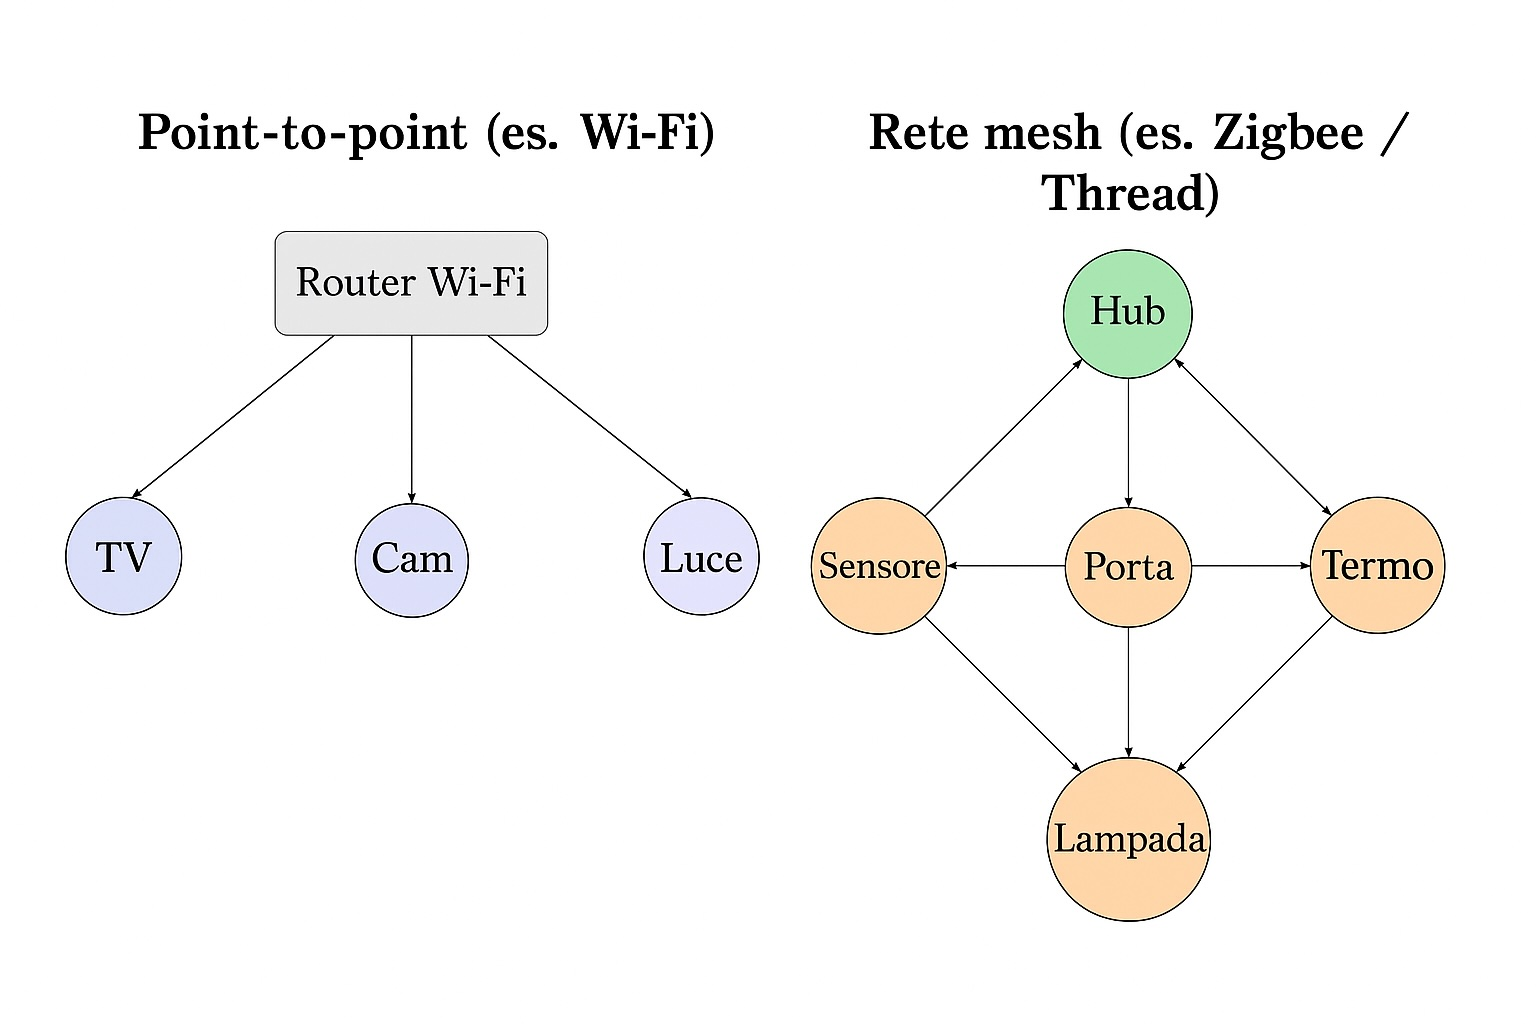
\includegraphics[scale=0.3]{immagini/reti.jpeg}
    \caption{Interfaccia Apple Home con dispositivi configurati}
    \label{fig:reti-mesh}
\end{figure}

In definitiva, quando si progettano sistemi domotici destinati a durare nel tempo e ad adattarsi a contesti mutevoli, scegliere protocolli con meccanismi di recupero e adattamento diventa una garanzia di stabilità e continuità.

\section{Confronto prestazionale tra Zigbee, Z-Wave, Wi-Fi, Thread e Matter}

\subsection{Zigbee: il veterano delle reti mesh}

Zigbee è considerato uno dei protocolli più consolidati nell’ambito della domotica, grazie alla sua lunga presenza sul mercato e alla vasta adozione da parte dei produttori. Basato sullo standard IEEE 802.15.4, opera principalmente sulla banda a 2.4 GHz, la stessa condivisa con Wi-Fi e Bluetooth.

\textbf{Punti di forza:}
\begin{itemize}
    \item Ecosistema maturo con ampia disponibilità di dispositivi
    \item Supporto per reti mesh auto-riparanti fino a 65.000 nodi teorici
    \item Profili applicativi standardizzati (es. Zigbee Home Automation, Zigbee Light Link)
    \item Consumi energetici estremamente ridotti
\end{itemize}

\textbf{Limitazioni:}
\begin{itemize}
    \item Rischio di interferenze nella banda 2.4 GHz
    \item Complessità nella gestione di reti molto estese
    \item Frammentazione tra profili e versioni differenti
    \item Velocità non adatta a trasferimenti di dati intensivi
\end{itemize}

Philips Hue, ad esempio, utilizza Zigbee per controllare fino a 50 lampadine con un singolo bridge, offrendo sincronizzazione precisa e latenza impercettibile.

\subsection{Z-Wave: l'alternativa su frequenze dedicate}

Z-Wave si distingue per l’utilizzo di frequenze sub-GHz (868 MHz in Europa, 908 MHz negli USA), che garantiscono una maggiore penetrazione attraverso muri e ridotte interferenze rispetto alla banda 2.4 GHz.

\textbf{Caratteristiche distintive:}
\begin{itemize}
    \item Interoperabilità certificata tra dispositivi Z-Wave
    \item Portata estesa fino a 100 metri in campo aperto
    \item Topologia mesh con routing source-routed ottimizzato
    \item Limite di 232 nodi per rete, sufficiente per l’ambito residenziale
\end{itemize}

La sua velocità massima, pari a 100 kbps, lo rende inadatto a carichi di dati elevati, ma perfetto per sistemi di controllo. Un impianto di sicurezza domestica può includere sensori di movimento, contatti magnetici per porte/finestre e sirene ad alta affidabilità.

\subsection{Wi-Fi: potenza e versatilità}

Il Wi-Fi domina per capacità di banda e diffusione. La presenza capillare di router domestici riduce la necessità di infrastrutture dedicate, rendendolo ideale per dispositivi che richiedono elevato throughput.

\textbf{Vantaggi competitivi:}
\begin{itemize}
    \item Larghezza di banda elevatissima, adatta a video e trasferimenti intensivi
    \item Infrastruttura già presente nella maggior parte delle abitazioni
    \item Supporto IP nativo, ideale per integrazione cloud
    \item Ottimizzazioni recenti in Wi-Fi 6 per dispositivi IoT (es. Target Wake Time)
\end{itemize}

\textbf{Sfide operative:}
\begin{itemize}
    \item Consumo energetico elevato, inadatto a dispositivi a batteria
    \item Degrado prestazionale con molti dispositivi connessi a un singolo access point
    \item Latenza variabile in presenza di congestione di rete
    \item Hardware più costoso rispetto ad alternative low-power
\end{itemize}

Le videocamere IP rappresentano un'applicazione ideale: richiedono banda elevata e sono alimentate da rete elettrica, eliminando il vincolo energetico \cite{WiFiVsIoT}.

\subsection{Thread: l'evoluzione IP-native}

Thread è un protocollo mesh moderno progettato per supportare IPv6 nativamente, con un’architettura leggera e sicura adatta all’era dell’interoperabilità e del cloud.

\textbf{Innovazioni chiave:}
\begin{itemize}
    \item Supporto IPv6 nativo con instradamento end-to-end
    \item Sicurezza avanzata con crittografia AES e gestione automatica delle chiavi
    \item Commissioning semplice via smartphone
    \item Mesh self-healing con tempi di riconvergenza rapidi
\end{itemize}

Le sue latenze sono paragonabili a Zigbee (20–50 ms), ma con un’architettura più moderna e scalabile. Dispositivi come Apple HomePod mini o Google Nest Hub fungono da border router per reti Thread, facilitando l’adozione senza componenti aggiuntivi \cite{thread-spec}.

\subsection{Matter: l’unificatore dell’ecosistema}

Matter si propone come livello applicativo universale, operando sopra protocolli esistenti come Thread, Wi-Fi ed Ethernet. Il suo obiettivo è garantire interoperabilità trasparente tra piattaforme e produttori.

\textbf{Punti di forza:}
\begin{itemize}
    \item Compatibilità trasversale tra Apple, Google, Amazon, Samsung
    \item Sicurezza integrata nel design, con certificazione obbligatoria
    \item Commissioning tramite QR code o NFC
    \item Comunicazione locale senza necessità di cloud
\end{itemize}

Matter introduce un overhead minimo (circa 5–10\% di latenza aggiuntiva), ma il vantaggio in termini di compatibilità compensa ampiamente. Un termostato compatibile può essere gestito indistintamente da Siri, Google Assistant o Alexa, mantenendo la stessa qualità d’interazione \cite{MatterWhitePaper}.

\begin{table}[htbp]
\centering
\begin{tabular}{|l|c|c|c|c|c|}
\hline
\textbf{Parametro} & \textbf{Zigbee} & \textbf{Z-Wave} & \textbf{Wi-Fi} & \textbf{Thread} & \textbf{Matter} \\
\hline
Banda & 2.4 GHz & Sub-GHz & 2.4/5 GHz & 2.4 GHz & - \\
Topologia & Mesh & Mesh & Point-to-point & Mesh & - \\
Velocità max & 250 kbps & 100 kbps & \textgreater100 Mbps & 250 kbps & - \\
Energia & Molto bassa & Bassa & Alta & Bassa & Variabile \\
Interoperabilità & Limitata & Alta (cert.) & Variabile & Alta & Massima \\
\hline
\end{tabular}
\caption{Confronto sintetico tra protocolli e standard IoT in ambito domotico}
\label{tab:confronto-protocolli}
\end{table}

\section{Scalabilità dei protocolli in ambienti domestici complessi}

Man mano che le abitazioni intelligenti si arricchiscono di sensori, attuatori e dispositivi di controllo, il tema della \textbf{scalabilità} diventa centrale. Un sistema domotico moderno non si limita più ad accendere qualche luce o a regolare il termostato: può arrivare a gestire centinaia di elementi distribuiti in ambienti ampi e strutturati. In questo contesto, è fondamentale comprendere come i principali protocolli IoT reagiscano all’aumento della complessità della rete.

\subsection{Scalabilità per protocollo}

\subsubsection{Zigbee: tra teoria e realtà}

Zigbee dichiara il supporto fino a 65.000 dispositivi per rete, un numero che, sulla carta, garantirebbe ampie possibilità di espansione. Tuttavia, in ambito residenziale, questa soglia è ben lontana dalla realtà operativa.

Già superata la soglia dei 200-300 dispositivi, cominciano a emergere difficoltà pratiche:
\begin{itemize}
    \item Latenze maggiori dovute al routing tra nodi multipli
    \item Congestione nella banda a 2.4 GHz, soprattutto in ambienti densi
    \item Rallentamenti durante aggiornamenti firmware distribuiti
    \item Complessità crescente nella configurazione e manutenzione
\end{itemize}

Una strategia spesso adottata è la creazione di \textbf{sotto-reti logiche} distinte, ciascuna gestita da un coordinator dedicato, per esempio separando l’illuminazione dalla climatizzazione o dai sistemi di sicurezza.

\subsubsection{Z-Wave: solido entro i propri limiti}

Z-Wave ha un limite teorico molto più contenuto: 232 dispositivi per rete. Tuttavia, per la maggior parte delle abitazioni — anche quelle di grandi dimensioni — si tratta di un numero più che sufficiente. La gestione più semplice e il minor rischio di congestione radio, grazie all’uso della banda sub-GHz, lo rendono una scelta solida e prevedibile.

Un'abitazione con circa 100 dispositivi (tra interruttori, sensori e attuatori) rientra tranquillamente nei limiti del protocollo, offrendo ancora margine per ulteriori espansioni.

\subsubsection{Thread e Matter: progettati per crescere}

Thread è stato pensato fin dall’inizio per reti scalabili, affidabili e facilmente gestibili:
\begin{itemize}
    \item I router mesh distribuiti bilanciano il traffico in modo dinamico
    \item L'uso nativo di IPv6 semplifica il routing e la gestione
    \item La rete si auto-configura e auto-ripara in caso di guasti
\end{itemize}

Test su installazioni reali mostrano che anche con oltre 200 dispositivi, i tempi di risposta restano sotto i 100 ms nel 95° percentile, con una degradazione molto graduale delle prestazioni all’aumentare del carico.

Matter, appoggiandosi a Thread (e in parte al Wi-Fi), eredita e potenzia questa capacità, offrendo al tempo stesso interoperabilità tra ecosistemi e gestione centralizzata semplificata.

\subsection{Strategie di progettazione per reti complesse}

\subsubsection{Progettare la rete per livelli}

Quando i dispositivi aumentano, progettare in modo gerarchico diventa essenziale. Una buona architettura divide la rete in tre livelli logici:

\begin{enumerate}
    \item \textbf{Livello Edge}: i dispositivi periferici (sensori, attuatori) che eseguono compiti specifici
    \item \textbf{Livello di Aggregazione}: hub locali o controller di zona che raccolgono e instradano i dati
    \item \textbf{Livello Core}: un controller principale (o cloud gateway) che integra, elabora e coordina tutto il sistema
\end{enumerate}

Questa suddivisione migliora la stabilità, semplifica la manutenzione e consente di isolare eventuali malfunzionamenti, evitando che si propaghino all’intero sistema.

\subsubsection{Separare per funzione: la rete è più leggibile}

Un'altra strategia efficace è la suddivisione dei dispositivi in reti logiche in base alla loro funzione:

\begin{itemize}
    \item \textbf{Rete Sicurezza}: dispositivi critici come sensori di movimento, allarmi e serrature (dove l'affidabilità è prioritaria)
    \item \textbf{Rete Comfort}: luci, termostati e tapparelle (ottimizzati per reattività e basso consumo)
    \item \textbf{Rete Media}: smart TV, speaker, videocamere (dove la banda e la connessione stabile sono fondamentali)
\end{itemize}

In questo modo si ottimizzano i protocolli per ciascun gruppo: Z-Wave può essere usato per la sicurezza, Zigbee o Thread per l’illuminazione, e il Wi-Fi per streaming e intrattenimento.

\subsection{Conclusioni sulla scalabilità}

In sostanza quando ci troviamo a realizzazione di sistemi domotici complessi, la prima vera sfida è quella della scalabilità che non si esaurisce nei soli numeri dichiarati dai produttori. Al contrario, deve essere fondamentale che la rete sia in grado di mantenere buoni tempi di risposta, sia semplice nella gestione ed affidabilità, sopratutto  quando il numero di dispositivi collegati aumenta sensibilmente.\\

Ogni protocollo che abbiamo visto finoea presenta caratteristiche diverse in questo scenario.\\
Zigbee può scalare bene, ma richiede una buona esperienza nella progettazione di rete per evitare colli di bottiglia.\\
Z-Wave, per la sua semplicità di configurazione e la sua stabilità, ottenuta sfruttando le banda sub-GHz con meno traffico, si adatta perfettamente a contesti residenziali di dimensioni medio-piccole.\\
Thread e Matter, diversamente dai precedenti, offrono un approccio più moderno e flessibile, risultando particolarmente indicati per installazioni più grandi, complesse e in continua evoluzione, spinto anche dall'innovazione che le proncipali aziende stanno dando a questo protocollo.\\

In conclusione, per definire il successo di una rete domotica complessa e grande, non bisogna guardare solo dal protocollo che abbiamo scelto, ma soprattutto da come viene disegnata: una buona progettazione, cola presenza di segmentazioni funzionali, la definizione di una organizzazione gerarchica, consentono di ottenere risultati affidabili e duraturi, qualunque sia la tecnologia utilizzata.

\chapter{Prospettive Future nella Domotica Residenziale}
\section{Il ruolo dello standard Matter e dei protocolli basati su IP}
Matter rappresenta una svolta nel panorama della domotica residenziale: è uno standard aperto sviluppato dalla Connectivity Standards Alliance (CSA) per garantire l'interoperabilità tra dispositivi di produttori diversi. Basato su protocolli IP, Matter consente una comunicazione sicura ed efficiente tra dispositivi domestici smart, eliminando molte delle barriere imposte dai sistemi proprietari. L'adozione su larga scala di Matter potrebbe uniformare il mercato e semplificare le configurazioni per l'utente finale \parencite{matterCSA}.

\section{Sviluppi tecnologici emergenti}

\subsection{Intelligenza artificiale e apprendimento automatico nella smart home}
L'integrazione dell'intelligenza artificiale (IA) nelle smart home è destinata a rivoluzionare l'automazione domestica. Sistemi basati su IA sono in grado di apprendere le abitudini dell'utente, anticiparne i bisogni e adattare dinamicamente le automazioni in funzione dei comportamenti rilevati. Questo approccio incrementa l'efficienza energetica, la personalizzazione e la sicurezza dei sistemi domotici \parencite{ieeeAI}.

\subsection{Reti mesh e Wi-Fi 6}
Le reti mesh rappresentano una soluzione sempre più diffusa per migliorare la copertura e l'affidabilità delle comunicazioni wireless in ambito domestico. In parallelo, la diffusione del Wi-Fi 6 porta significativi miglioramenti in termini di velocità, efficienza e capacità di gestire un elevato numero di dispositivi contemporaneamente, rendendolo particolarmente adatto a contesti smart home complessi \parencite{etsiWifi6}.

\section{Sfide legate alla privacy e alla sicurezza}
Con l'aumento dei dispositivi connessi cresce anche il rischio legato alla sicurezza informatica. I sistemi domotici sono potenziali bersagli di attacchi hacker e possono comportare violazioni della privacy. Tra le principali criticità si evidenziano:
\begin{itemize}
    \item trasmissione non cifrata di dati sensibili;
    \item vulnerabilità nei firmware dei dispositivi;
    \item accessi non autorizzati tramite reti domestiche compromesse.
\end{itemize}

Per affrontare tali sfide, sono fondamentali l'adozione di protocolli sicuri, aggiornamenti software regolari, e la consapevolezza dell'utente riguardo le buone pratiche di cybersicurezza \parencite{nistIotSecurity}.



\chapter{Prospettive Future nella Domotica Residenziale}
\section{Il ruolo dello standard Matter e dei protocolli basati su IP}
Matter rappresenta una svolta nel panorama della domotica residenziale: è uno standard aperto sviluppato dalla Connectivity Standards Alliance (CSA) per garantire l'interoperabilità tra dispositivi di produttori diversi. Basato su protocolli IP, Matter consente una comunicazione sicura ed efficiente tra dispositivi domestici smart, eliminando molte delle barriere imposte dai sistemi proprietari. L'adozione su larga scala di Matter potrebbe uniformare il mercato e semplificare le configurazioni per l'utente finale \parencite{matterCSA}.

\section{Sviluppi tecnologici emergenti}

\subsection{Intelligenza artificiale e apprendimento automatico nella smart home}
L'integrazione dell'intelligenza artificiale (IA) nelle smart home è destinata a rivoluzionare l'automazione domestica. Sistemi basati su IA sono in grado di apprendere le abitudini dell'utente, anticiparne i bisogni e adattare dinamicamente le automazioni in funzione dei comportamenti rilevati. Questo approccio incrementa l'efficienza energetica, la personalizzazione e la sicurezza dei sistemi domotici \parencite{ieeeAI}.

\subsection{Reti mesh e Wi-Fi 6}
Le reti mesh rappresentano una soluzione sempre più diffusa per migliorare la copertura e l'affidabilità delle comunicazioni wireless in ambito domestico. In parallelo, la diffusione del Wi-Fi 6 porta significativi miglioramenti in termini di velocità, efficienza e capacità di gestire un elevato numero di dispositivi contemporaneamente, rendendolo particolarmente adatto a contesti smart home complessi \parencite{etsiWifi6}.

\section{Sfide legate alla privacy e alla sicurezza}
Con l'aumento dei dispositivi connessi cresce anche il rischio legato alla sicurezza informatica. I sistemi domotici sono potenziali bersagli di attacchi hacker e possono comportare violazioni della privacy. Tra le principali criticità si evidenziano:
\begin{itemize}
    \item trasmissione non cifrata di dati sensibili;
    \item vulnerabilità nei firmware dei dispositivi;
    \item accessi non autorizzati tramite reti domestiche compromesse.
\end{itemize}

Per affrontare tali sfide, sono fondamentali l'adozione di protocolli sicuri, aggiornamenti software regolari, e la consapevolezza dell'utente riguardo le buone pratiche di cybersicurezza \parencite{nistIotSecurity}.



\chapter{Caso di Studio: Sistema Domotico Integrato con Apple HomeKit}

\section{Obiettivi e contesto}
Questo caso di studio documenta l’implementazione di un sistema domotico per una residenza unifamiliare su due piani, integrato nativamente con Apple HomeKit. 

I requisiti riguardano: (i) controllo accessi sicuro; (ii) gestione dell’illuminazione e delle tapparelle; (iii) videosorveglianza perimetrale con notifiche mirate; (iv) monitoraggio ambientale e automazioni meteo; (v) audio multi stanza; (vi) facilità d’uso tramite app Casa e comandi vocali; (vii) riduzione dei consumi energetici senza impattare il comfort.

\section{Analisi dell’abitazione}
\textbf{Piano terra} (100 m²): ingresso, soggiorno open-space (40 m²), cucina abitabile (25 m²), bagno ospiti, studio/ufficio (15 m²), garage doppio.\\
\textbf{Piano primo} (100 m²): camera matrimoniale con bagno, due camere singole, bagno principale, terrazzo (20 m²).\\
\textbf{Esterno}: giardino perimetrale, vialetto d’accesso, due accessi carrabili, area barbecue.

Vincoli progettuali: distribuzione su due piani (copertura Wi‑Fi e latenza), esposizioni est/ovest (controllo solare), necessità di integrazione non invasiva su impianto esistente e preferenza per controllo nativo da ecosistema Apple. Facilità di gestione e condivisione con i membri della famiglia.

\section{Architettura del sistema}
L’architettura è organizzata su tre livelli: (a) \textit{dispositivi e sensori}; (b) \textit{hub/controller e gateway}; (c) \textit{automazioni e interfacce}.

\subsection{Rete e infrastruttura}
\begin{itemize}
  \item \textbf{LAN IoT dedicata}: VLAN 192.168.20.0/24, SSID dedicato (WPA3), segmentazione del traffico verso la LAN principale.
  \item \textbf{Hub HomeKit}: HomePod in soggiorno come hub primario; HomePod mini in cucina, studio e camera matrimoniale come hub di failover e per audio locale.
  \item \textbf{Gateway BTicino}: modulo DIN collegato alla rete Wi-Fi per la configurazione dei dispositivi su home control e condivisione con HomeKit.
\end{itemize}

\subsection{Protocolli e integrazione}
\begin{itemize}
  \item \textbf{Bus SCS (BTicino)}: utilizzato per la comunicazione tra moduli Living Now cablati (interruttori, dimmer e comandi tapparelle) e il gateway, quando l’impianto lo prevede. Garantisce bassa latenza e funzionalità anche in assenza di rete IP.
  \item \textbf{Wi-Fi}: impiegato dai dispositivi Living Now connessi \textit{pre-Matter} (installati in questa abitazione), dal Nuki Smart Lock 3.0 Pro, dalle telecamere Netatmo e dalla stazione meteo Netatmo. È il principale canale di comunicazione verso HomeKit in questa configurazione.
  \item \textbf{Thread}: utilizzato esclusivamente da dispositivi compatibili Matter o nativamente Thread, come le Nanoleaf Lines. La rete Thread è gestita dai Border Router integrati in HomePod mini e HomePod (2ª gen), garantendo bassa latenza e consumo energetico ridotto.
  \item \textbf{Interruttori BTicino wireless}: modelli da parete privi di cablaggio, alimentati a batteria con comunicazione radio diretta con il gateway via Thread.
  \item \textbf{HomeKit su IP}: protocollo applicativo utilizzato per automazioni e controlli, con cifratura end-to-end e pairing tramite codice QR.
  \item \textbf{HomeKit Secure Video (HKSV)}: per le telecamere Netatmo, con analisi video on-device e registrazione cifrata su iCloud.
\end{itemize}

\section{Dotazione installata (per categoria)}
\subsection*{Accesso e sicurezza}
\begin{itemize}
  \item \textbf{Serratura smart}: Nuki Smart Lock 3.0 Pro (integrazione HomeKit via Wi‑Fi). Funzioni: blocco/sblocco, stato porta, automazioni in base a presenza e orario. La gestione delle credenziali ospiti avviene nell’app Nuki; HomeKit fornisce controllo e notifiche.
  \item \textbf{Videosorveglianza esterna}: 4 telecamere Netatmo Outdoor con sirena. In HomeKit Secure Video: rilevamento persone/animali/veicoli, zone di attività, timeline cifrata. Posizionamento: ingresso, garage, giardino posteriore, lato secondario.
\end{itemize}

\subsection*{Illuminazione e schermature}
\begin{itemize}
  \item \textbf{Punti luce e dimmer}: serie BTicino Living Now per 32 punti luce (on/off e dimmerazione). Comandi scenari locali per richiamo rapido.
  \item \textbf{Tapparelle}: 18 motorizzazioni con controllo salita/discesa/stop e posizionamento percentuale; scenari alba/tramonto.
\end{itemize}

\subsection*{Monitoraggio ambientale e meteo}
\begin{itemize}
  \item \textbf{Stazione meteo Netatmo}: modulo interno (temperatura, umidità, CO\textsubscript{2}, pressione, rumore) e modulo esterno (temperatura/umidità). Dati usati per automazioni (protezione solare, avvisi vento/calore).
  \item \textbf{Sensori integrati HomePod}: temperatura/umidità ambientale disponibili in HomeKit per regole semplici di comfort.
\end{itemize}

\subsection*{Audio, interazione e notifiche}
\begin{itemize}
  \item \textbf{HomePod / HomePod mini}: audio multi-room, comandi vocali, Intercom, hub HomeKit con failover. Integrazione con scene (es. modalità cinema, sveglia graduale).
\end{itemize}

\subsection*{Illuminazione decorativa}
\begin{itemize}
  \item \textbf{Nanoleaf Lines}: installazione a parete in soggiorno (dietro TV). Integrazione con HomeKit per scene; effetti dinamici per notifiche e modalità cinema. Connessione di rete via Wi‑Fi; supporto a protocolli low-latency ove disponibile.
\end{itemize}

\section{Implementazione}
\subsection{Fase 1 — Infrastruttura elettrica e di rete}
\begin{enumerate}
  \item Installazione del gateway BTicino su barra DIN e predisposizione protezioni dedicate.
  \item Alimentazioni per telecamere esterne.
  \item Configurazione VLAN/SSID IoT, indirizzamento statico per dispositivi fissi (telecamere, gateway), WPA3.
\end{enumerate}

\subsection{Fase 2 — Installazione dispositivi}
\begin{itemize}
  \item Sostituzione interruttori tradizionali con moduli Living Now; configurazione dimmer nelle zone principali; comandi tapparelle.
  \item Montaggio Nuki su porta blindata con calibrazione.
  \item Installazione telecamere Netatmo e definizione delle zone di attività.
  \item Posizionamento HomePod/HomePod mini e installazione Nanoleaf Lines.
\end{itemize}

\subsection{Fase 3 — Configurazione HomeKit}
\begin{enumerate}
  \item Aggiunta del gateway BTicino tramite codice HomeKit; rilevamento automatico dei dispositivi collegati.
  \item Pairing di telecamere e stazione meteo Netatmo; abilitazione HKSV.
  \item Configurazione Nuki via QR e verifica controlli da app Casa.
  \item Impostazione HomePod come hub primario e verifica dei servizi remoti.
  \item Organizzazione in stanze/piani e definizione di zone (interno/esterno).
\end{enumerate}

\section{Automazioni rappresentative}
Le automazioni sono progettate con logica "\textit{evento-condizione-azione}", utilizzando trigger affidabili e preferendo esecuzione locale quando possibile.

\subsection*{Protezione notturna}
\begin{verbatim}
Trigger: tramonto + 30 min; presenza = true
Azioni: chiusura tapparelle piano terra; accensione luci esterne;
        telecamere in alta sensibilità; blocco automatico serratura.
Notifiche: sintesi eventi su iPhone dei genitori.
\end{verbatim}

\subsection*{Arrivo familiare (riconoscimento)}
\begin{verbatim}
Trigger: Netatmo ingresso -> persona riconosciuta; fascia oraria: 18:00-23:00
Azioni: luce ingresso 100% a 3000K; avviso su HomePod (Intercom);
        sblocco manuale facilitato (notifica azionabile da Apple Watch/iPhone).
\end{verbatim}

\subsection*{Ottimizzazione solare estiva}
\begin{verbatim}
Trigger: temperatura esterna > 26°C; meteo soleggiato
Condizioni: stagione = estate; qualcuno in casa = true
Azioni progressive: lato est 70% (10:00); lato sud 80% (12:00);
                   lato ovest 70% (15:00); apertura al tramonto.
\end{verbatim}

\subsection*{Sveglia graduale}
\begin{verbatim}
Trigger: 07:00 (feriali) / 08:30 (weekend)
Azioni: tapparelle camera 30% con apertura lenta; luce 20% a 2700K (5 min);
        HomePod: riproduzione playlist con volume in fade-in.
\end{verbatim}

\subsection*{Modalità cinema}
\begin{verbatim}
Trigger: comando vocale "Ehi Siri, modalità cinema" o pulsante scena
Azioni: chiusura tapparelle soggiorno; spegnimento luci;
        Nanoleaf Lines in Screen/Mirror a 30%;
        HomePod in modalità Home Theater; notifiche familiari silenziate (2 ore).
\end{verbatim}

\section{Gestione utenti, permessi e privacy}
\begin{itemize}
  \item \textbf{Ruoli HomeKit}: genitori come amministratori (gestione dispositivi, automazioni, registrazioni video); figli come membri con accesso a luci/tapparelle e audio nelle loro stanze; esclusi controlli su serratura e telecamere.
  \item \textbf{HKSV e dati}: analisi movimento on-device, video cifrati end-to-end con storage iCloud; definizione di zone sensibili per ridurre notifiche superflue.
  \item \textbf{Accessi ospiti}: gestione credenziali temporanee tramite app Nuki; revoca immediata; log accessi consultabile.
\end{itemize}

\section{Conclusioni: vantaggi dell'integrazione multimarca}
L'adozione di un'architettura HomeKit in un contesto multimarca, come quello descritto in questo caso di studio, ha permesso di ottenere un impianto coerente, sicuro e facile da gestire.

\paragraph{Principali vantaggi osservati}
\begin{itemize}
  \item \textbf{Gestione centralizzata}: controllo di dispositivi BTicino, Netatmo, Nuki e Nanoleaf da un'unica interfaccia (app Casa), senza necessità di app separate per l'uso quotidiano su ogni device.
  \item \textbf{Condivisione semplificata}: accesso esteso a tutti i membri della famiglia tramite Condivisione in famiglia Apple, senza configurazioni aggiuntive.
  \item \textbf{Privacy e sicurezza}: automazioni locali e cifratura end-to-end nativa di HomeKit; per i video, HomeKit Secure Video con analisi on-device e archiviazione cifrata.
  \item \textbf{Riduzione della complessità}: eliminazione di gateway e bridge multipli, con aggiornamenti e notifiche centralizzati.
  \item \textbf{Affidabilità operativa}: continuità di funzionamento locale per luci, tapparelle e scenari principali anche in assenza di connessione Internet.
  \item \textbf{Esperienza uniforme}: interfaccia e comandi vocali coerenti su iPhone, iPad, Mac e Apple Watch.
  \item \textbf{Scalabilità futura}: predisposizione della rete per dispositivi Matter/Thread, grazie alla presenza di border router integrati (HomePod).
  \item \textbf{Efficienza energetica}: automazioni di illuminazione e schermature solari che contribuiscono alla riduzione dei consumi e al miglioramento del comfort abitativo.
  \item \textbf{Maggiore sicurezza di rete}: segmentazione VLAN dedicata all'IoT e isolamento del traffico rispetto alla rete principale.
\end{itemize}

\noindent In sintesi, la soluzione implementata dimostra come un ecosistema aperto e interoperabile, basato su standard consolidati come HomeKit, possa integrare tecnologie di produttori diversi garantendo facilità d'uso, sicurezza e possibilità di evoluzione nel tempo.
\appendix
\chapter{Glossario dei termini e degli acronimi}
\begin{description}
    \item[IoT] Internet of Things --- Insieme di dispositivi interconnessi che comunicano tra loro via rete.
    \item[Smart Home] Abitazione intelligente in cui dispositivi e impianti sono automatizzati e controllabili a distanza.
    \item[BLE] Bluetooth Low Energy --- Standard wireless a basso consumo energetico.
    \item[Zigbee] Protocollo wireless basato su IEEE 802.15.4, ottimizzato per reti mesh a corto raggio.
    \item[Z-Wave] Protocollo wireless a bassa potenza, usato per applicazioni di domotica.
    \item[Wi-Fi] Wireless Fidelity --- Tecnologia di rete locale senza fili basata su IEEE 802.11.
    \item[Thread] Protocollo di rete IPv6-based pensato per dispositivi IoT.
    \item[Matter] Standard aperto per l'interoperabilità tra dispositivi smart, sviluppato dalla CSA.
    \item[HomeKit] Framework Apple per l'integrazione e gestione di dispositivi smart home.
    \item[Gateway] Dispositivo che consente la comunicazione tra reti o protocolli differenti.
    \item[API] Application Programming Interface --- Interfaccia che permette l'interazione tra software.
    \item[Hub] Dispositivo centrale che coordina il traffico e l'automazione dei dispositivi smart.
    \item[CSA] Connectivity Standards Alliance --- Organismo che promuove standard aperti per l'IoT.
    \item[NIST] National Institute of Standards and Technology --- Agenzia USA per standard e tecnologie.

    \item[KNX] Standard aperto per l'automazione degli edifici, utilizzato principalmente in sistemi cablati per applicazioni domotiche.
    \item[NIST IoT Security] Linee guida e best practice sulla sicurezza IoT definite dal National Institute of Standards and Technology.


    \item[RS-485] Standard di comunicazione seriale cablato, resistente alle interferenze e utilizzato principalmente in ambienti industriali e domotici per connessioni su lunghe distanze.
    \item[Bluetooth Low Energy (BLE)] Versione del protocollo Bluetooth a basso consumo energetico, particolarmente adatta per dispositivi IoT con alimentazione a batteria.

    \item[VLAN] Virtual Local Area Network --- Una rete logica separata all'interno della stessa infrastruttura fisica, utilizzata per segmentare e proteggere la rete domestica.
    \item[IDS] Intrusion Detection System --- Sistema di monitoraggio del traffico di rete per individuare attività sospette o non autorizzate.
    \item[Firmware] Software installato su dispositivi hardware IoT, responsabile della gestione diretta delle funzionalità del dispositivo.
    \item[DTLS] Datagram Transport Layer Security --- Protocollo di sicurezza che fornisce comunicazioni cifrate per dispositivi con risorse limitate, basato su UDP.
    \item[Man-in-the-Middle (MitM)] Tipo di attacco informatico in cui un aggressore intercetta e potenzialmente manipola la comunicazione tra due dispositivi.

\end{description}

\printbibliography
\end{document}
